\documentclass[10pt]{article}\usepackage[margin=.7in]{geometry}\usepackage{graphicx}\begin{document}\section*{Independent word Add11 review}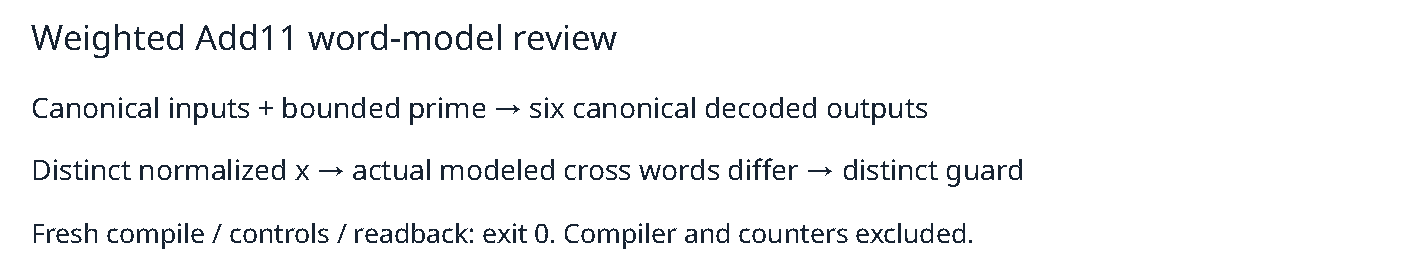
\includegraphics[width=\linewidth]{figure.pdf}
No blocking discrepancy was found for the stated literal-word-model correspondence. Producer hashes matched. Fresh module, controls and axiom readback compiled with exit zero; retained dependencies were reused.

\paragraph{Power loop} Exponent five follows 5,2,1,0: initial multiplication by one, two conditional squares, final accumulator multiplication. There is no trailing unused square. The exact unroll is reflexive.

\paragraph{Payload} Bounded canonical operands permit compositional modular-value decoding. All six payload words are canonical and decode to the reviewed weighted field formula. Expression sharing and operation counts are not established by this value model.

\paragraph{Dispatch} Inverse precedes doubling and then the equal-cross assertion. Distinct normalized x with nonzero decoded z excludes equal machine cross words, so the modeled distinct branch is selected.

\paragraph{Boundary} Field.n=1, no tables, odd-prime path and normal counter execution are source-mapping conditions. This is not compiled Rust equivalence, normalized word Mumford validity or a group-law/walk proof. No scientific trial or cost claim was produced. REVIEW.md and receipts.json retain details and exact checks.
\end{document}